\documentclass[a4paper,11pt,twoside]{scrartcl}
\usepackage[T1]{fontenc}
\usepackage[utf8]{inputenc}
\usepackage{ngerman, eucal, mathrsfs, amsfonts, bbm, amsmath, amssymb, stmaryrd, array, xcolor,graphicx, float, wrapfig}
\usepackage{epstopdf}
\usepackage{listings}
\usepackage[official]{eurosym}
\DeclareUnicodeCharacter{20AC}{\EUR{}}


\definecolor{middlegray}{rgb}{0.5,0.5,0.5}
\definecolor{lightgray}{rgb}{0.8,0.8,0.8}
\definecolor{orange}{rgb}{0.8,0.3,0.3}
\definecolor{yac}{rgb}{0.6,0.6,0.1}
\definecolor{green}{rgb}{0,.5,0}

\lstdefinestyle{c}{
	keywordstyle=\bfseries\ttfamily\color{blue},
	stringstyle=\color{orange}\ttfamily,
	commentstyle=\color{green}\ttfamily,
	emph={@Override, while, forall, if}, 
	emphstyle=\color{green}\texttt,
	emph={[2]List, Queue},
	emphstyle={[2]\color{yac}\texttt},
}
\lstset{
	basicstyle=\ttfamily,
	showstringspaces=false,
	flexiblecolumns=true,
	tabsize=2,
	numbers=left,
	numberstyle=\tiny,
	numberblanklines=false,
	stepnumber=1,
	numbersep=10pt,
	xleftmargin=15pt,
	breaklines=true,
	inputencoding=utf8
}

\lstdefinestyle{java}{
	language = java,
	emph={@Override}, 
	emphstyle=\color{teal}\texttt,
	emph={[2]Node,T,Comparable,AbstractNode,System, Thread,Random, Tree, Integer, Math, String, InterruptedException, Map, Entry, Point, TreeMap, PrintWriter, Scanner, FileReader, FileInputStream, FileNotFoundException, InputStreamReader, UnsupportedEncodingException, DecimalFormat, ArrayList, HashSet, LinkedList, IOException, HashMap, MapTest, MyHashMap, Puzzle, MyQueue, StringBuilder, NoSuchElementException, List, Queue, Vector, Tuple,Search, IllegalArgumentException, UnionFind, AbstractUnionFind, SpanningTree, Collections, WeightedEdge},
	emphstyle={[2]\color{yac}\texttt},
	texcl=true,
	keywordstyle=\color{blue}\ttfamily,
	stringstyle=\color{red}\ttfamily,
	commentstyle=\color{green}\ttfamily
}

\lstset{literate=
	{á}{{\'a}}1 {é}{{\'e}}1 {í}{{\'i}}1 {ó}{{\'o}}1 {ú}{{\'u}}1
	{Á}{{\'A}}1 {É}{{\'E}}1 {Í}{{\'I}}1 {Ó}{{\'O}}1 {Ú}{{\'U}}1
	{à}{{\`a}}1 {è}{{\`e}}1 {ì}{{\`i}}1 {ò}{{\`o}}1 {ù}{{\`u}}1
	{À}{{\`A}}1 {È}{{\'E}}1 {Ì}{{\`I}}1 {Ò}{{\`O}}1 {Ù}{{\`U}}1
	{ä}{{\"a}}1 {ë}{{\"e}}1 {ï}{{\"i}}1 {ö}{{\"o}}1 {ü}{{\"u}}1
	{Ä}{{\"A}}1 {Ë}{{\"E}}1 {Ï}{{\"I}}1 {Ö}{{\"O}}1 {Ü}{{\"U}}1
	{â}{{\^a}}1 {ê}{{\^e}}1 {î}{{\^i}}1 {ô}{{\^o}}1 {û}{{\^u}}1
	{Â}{{\^A}}1 {Ê}{{\^E}}1 {Î}{{\^I}}1 {Ô}{{\^O}}1 {Û}{{\^U}}1
	{œ}{{\oe}}1 {Œ}{{\OE}}1 {æ}{{\ae}}1 {Æ}{{\AE}}1 {ß}{{\ss}}1
	{ű}{{\H{u}}}1 {Ű}{{\H{U}}}1 {ő}{{\H{o}}}1 {Ő}{{\H{O}}}1
	{ç}{{\c c}}1 {Ç}{{\c C}}1 {ø}{{\o}}1 {å}{{\r a}}1 {Å}{{\r A}}1
	{€}{{\EUR}}1 {£}{{\pounds}}1
}
\usepackage{geometry}
\geometry{left=25mm, right=15mm, bottom=25mm}
\setlength{\parindent}{0em} 
\setlength{\headheight}{0em} 
\usepackage{eucal} %Matheschriften http://www.maths.usyd.edu.au/u/SMS/texdoc/euscript.pdf
\usepackage{mathrsfs} %schriften
\usepackage{amsfonts} %schriften https://www.ctan.org/pkg/amsfonts?lang=de
\usepackage{bbm} %Schriften http://mirrors.ctan.org/macros/latex/contrib/bbm/bbm.pdf
\usepackage{amsmath} %Mathezeug https://www.ctan.org/pkg/amsmath
\usepackage{amssymb} %Macros für Symbole https://www.ctan.org/pkg/amsfonts
\usepackage{stmaryrd} %Mehr Symbole ftp://ftp.rrzn.uni-hannover.de/pub/mirror/tex-archive/fonts/stmaryrd/stmaryrd.pdf

\newcommand{\grad}{\text{grad}}
\makeatletter
\g@addto@macro\bfseries{\boldmath} %Fette Mathe Symbole in Überschriften
\makeatother

\title{Datenstrukturen und effiziente Algorithmen\\ Blatt 12}
\author{Markus Vieth, David Klopp, Christian Stricker}
\date{\today}



\begin{document}

\maketitle
\cleardoublepage
\pagestyle{myheadings}
\markboth{Markus Vieth,  David Klopp, Christian Stricker}{Markus Vieth, David Klopp, Christian Stricker}

\section*{Aufgabe 1}
\subsection*{a)} 
Definiere zwei Farben (hier rot und blau)\\
Wähle einen beliebigen Knoten als ''CurrentVertex'' und setze ihn auf blau.\\

\begin{lstlisting}[basicstyle=\scriptsize\ttfamily]
Wiederhole {
	Füge alle Nachbarknoten in eine Warteschlange.
	Falls CurrentVertex blau und mindestens einer der Nachbarknoten auch blau {
		Rückgabe: FALSE
	} ansonsten {
		setze alle Nachbarknoten auf rot
	}
	
	Falls CurrentVertex rot und mindestens einer der Nachbarknoten auch rot {
		Rückgabe: FALSE
	} ansonsten {
		setze alle Nachbarknoten auf blau
	}
	Wähle den nächsten Knoten aus der Warteschlange als CurrentVertex
}

Falls die Liste leer ist {
	Rückgabe: TRUE
}
\end{lstlisting}

\subsection*{b)}
\subsubsection*{\footnotesize BipartiterGraph.java}
\lstinputlisting[style=java,basicstyle=\scriptsize\ttfamily]{Code/UndirectedGraph.java}
\lstinputlisting[style=java,basicstyle=\scriptsize\ttfamily]{Code/BipartiterGraph.java}


\section*{Aufgabe 2}
\subsection*{Behauptung}
Die Umdefinierung ändert nichts an den Aussagen in der Vorlesung
\subsection*{Beweis}
\subsubsection*{Aussage}
Alle Knoten in $\tilde{G}$ haben höchstens Grad 2, ansonsten wäre ein Knoten inzident zu zwei Kanten aus dem Gleichen Matching $M$ oder $M^*$.
\subsubsection*{Überprüfung}
An dieser Aussage ändert sich nichts. Man kann das gleiche Argument verwenden.

\subsubsection*{Aussage}
$\tilde{G}$ besteht aus einzelnen Knoten, Pfaden gerader oder ungerader Länge und Zyklen gerader Länge.
\subsubsection*{Überprüfung}
Die einzelnen Knoten sind trivial. Pfade gerader oder ungerader Länge, also Pfade im allgemeinen, können weiterhin bestehen. Auch Zykel können weiterhin entstehen, mit Ausnahme jener mit ungerader Länge, da hier jede Kante abwechselnd aus den Matchings stammen müsste. Dies geht aber nur für gerade Matchings auf. Die Vereinigung hat auch hier keine Auswirkung, da Knoten mit einer Kante aus der Schnittmenge nur den Grad 1 haben kann.

\subsubsection*{Aussage}
Es gibt in $\tilde{G}$ mindestens einen $M$-augmentierenden Pfad $p$, der mehr Kanten aus $M^*$ als aus $M$ besitzt. Dies gilt, weil ansonsten $|M^*| \leq |M|$
\subsubsection*{Überprüfung}
Auch diese Aussage gilt in beiden Fällen, unter der Annahme, dass man Kanten aus der Schnittmenge entweder gar nicht oder zu beiden Matchings zählt.
\section*{Aufgabe 3}
\subsection*{a)} 




\begin{center}
	{\scriptsize\vspace{-20pt}
  \begin{tabular}{| c || c | c | c |}
    \hline
    Knoten & Input & Output & Differenz\\ \hline
    0 & 12     & 5 + 7 & 0 \\ \hline
    1 & 5       & 5       & 0 \\ \hline
    2 &  9      & 6 + 3 & 0 \\ \hline
    3 & 6 +7  & 13     & 0 \\ \hline
    4 & 0       & 0       & 0 \\ \hline
    5 & 0 + 3 & 3       & 0 \\ \hline
  \end{tabular}
}
\end{center}

$ $\\

\begin{wrapfigure}{R}{0.65\linewidth}
	\centering
	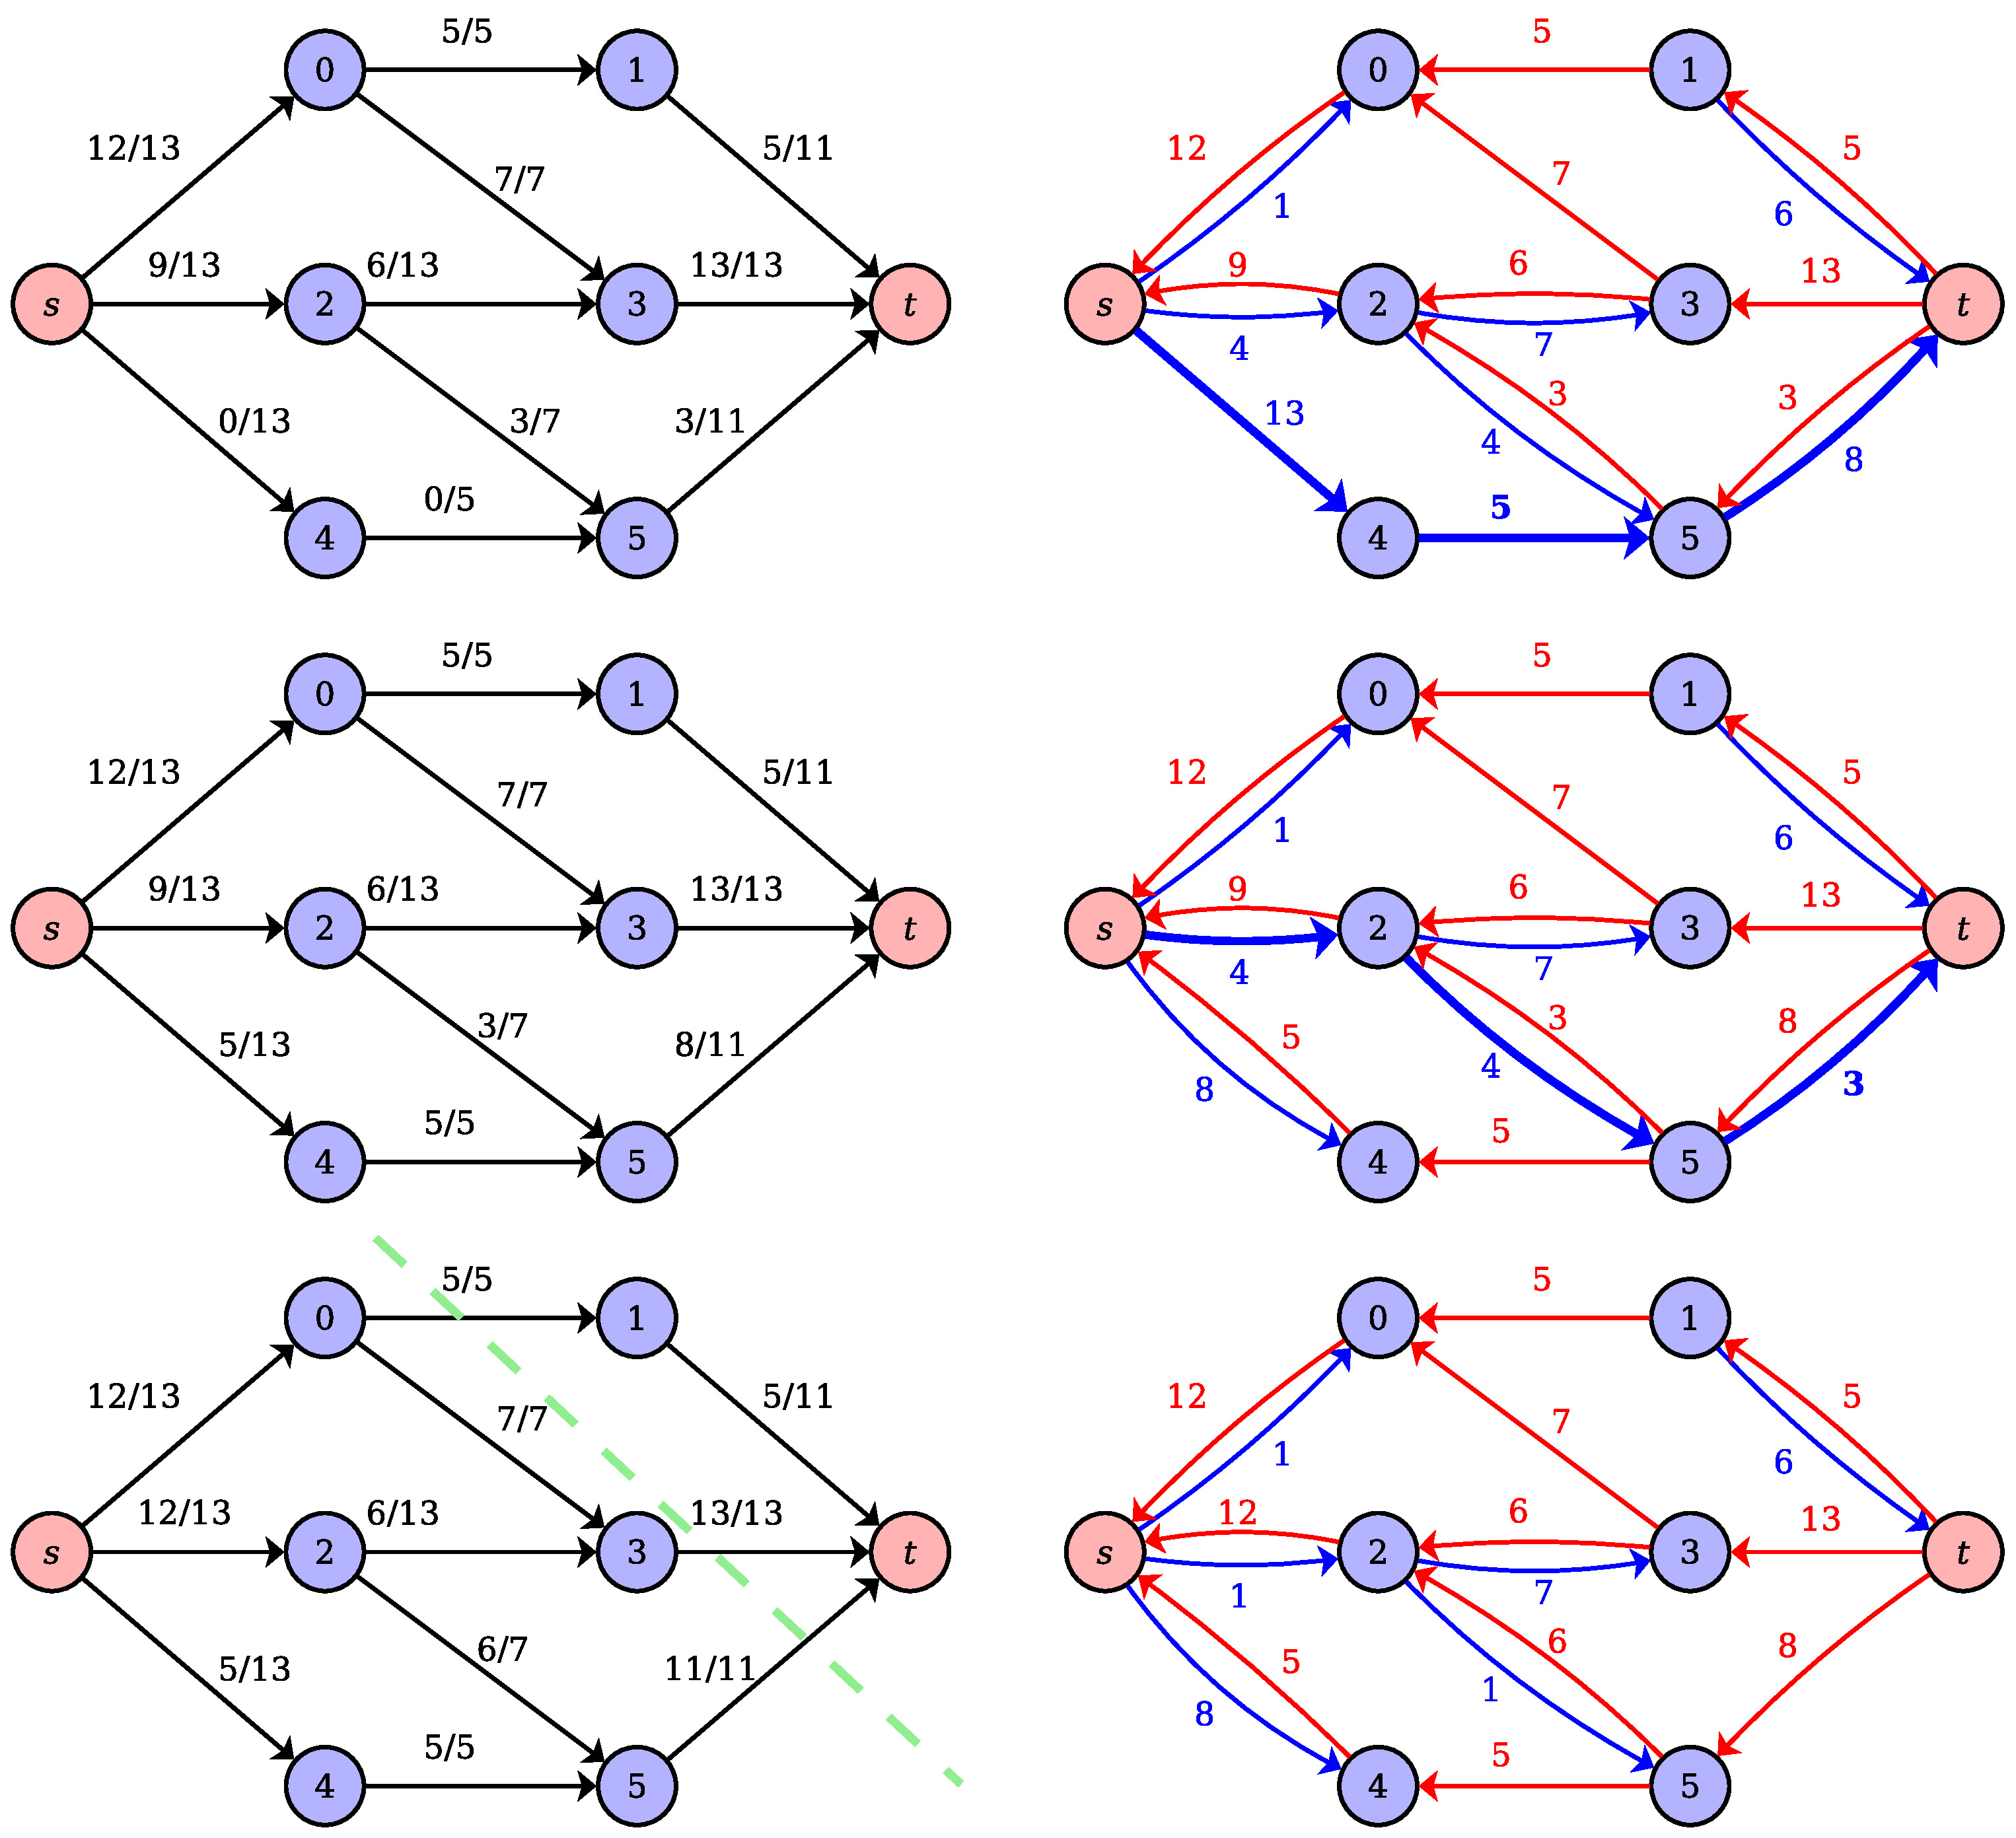
\includegraphics[width=0.9\linewidth]{Grafik/Diagramm1}
	\caption{Ford-Fulkerson}
	\label{fig:Ford-Fulkerson}
	\vspace*{-120pt}
\end{wrapfigure}

$ $\\

Der Input ist niemals größer als die maximale Kapazität. Für alle Knoten bis auf $s$ und $t$ stimmt die Anzahl des Inputs mit der des Outputs  überein. Es handelt sich daher um einen gültigen Fluss.
\subsection*{b)}
Nein, der eingezeichnete Fluss ist nicht maximal.
\subsection*{c)}
Siehe grüne, gestrichelte Linie. Der Schnitt geht durch die Kanten 0-1,3-t,5-t und entspricht dem maximalen Fluss (29).

\pagebreak

\subsection*{d)}

\begin{figure}[H]
	\centering
	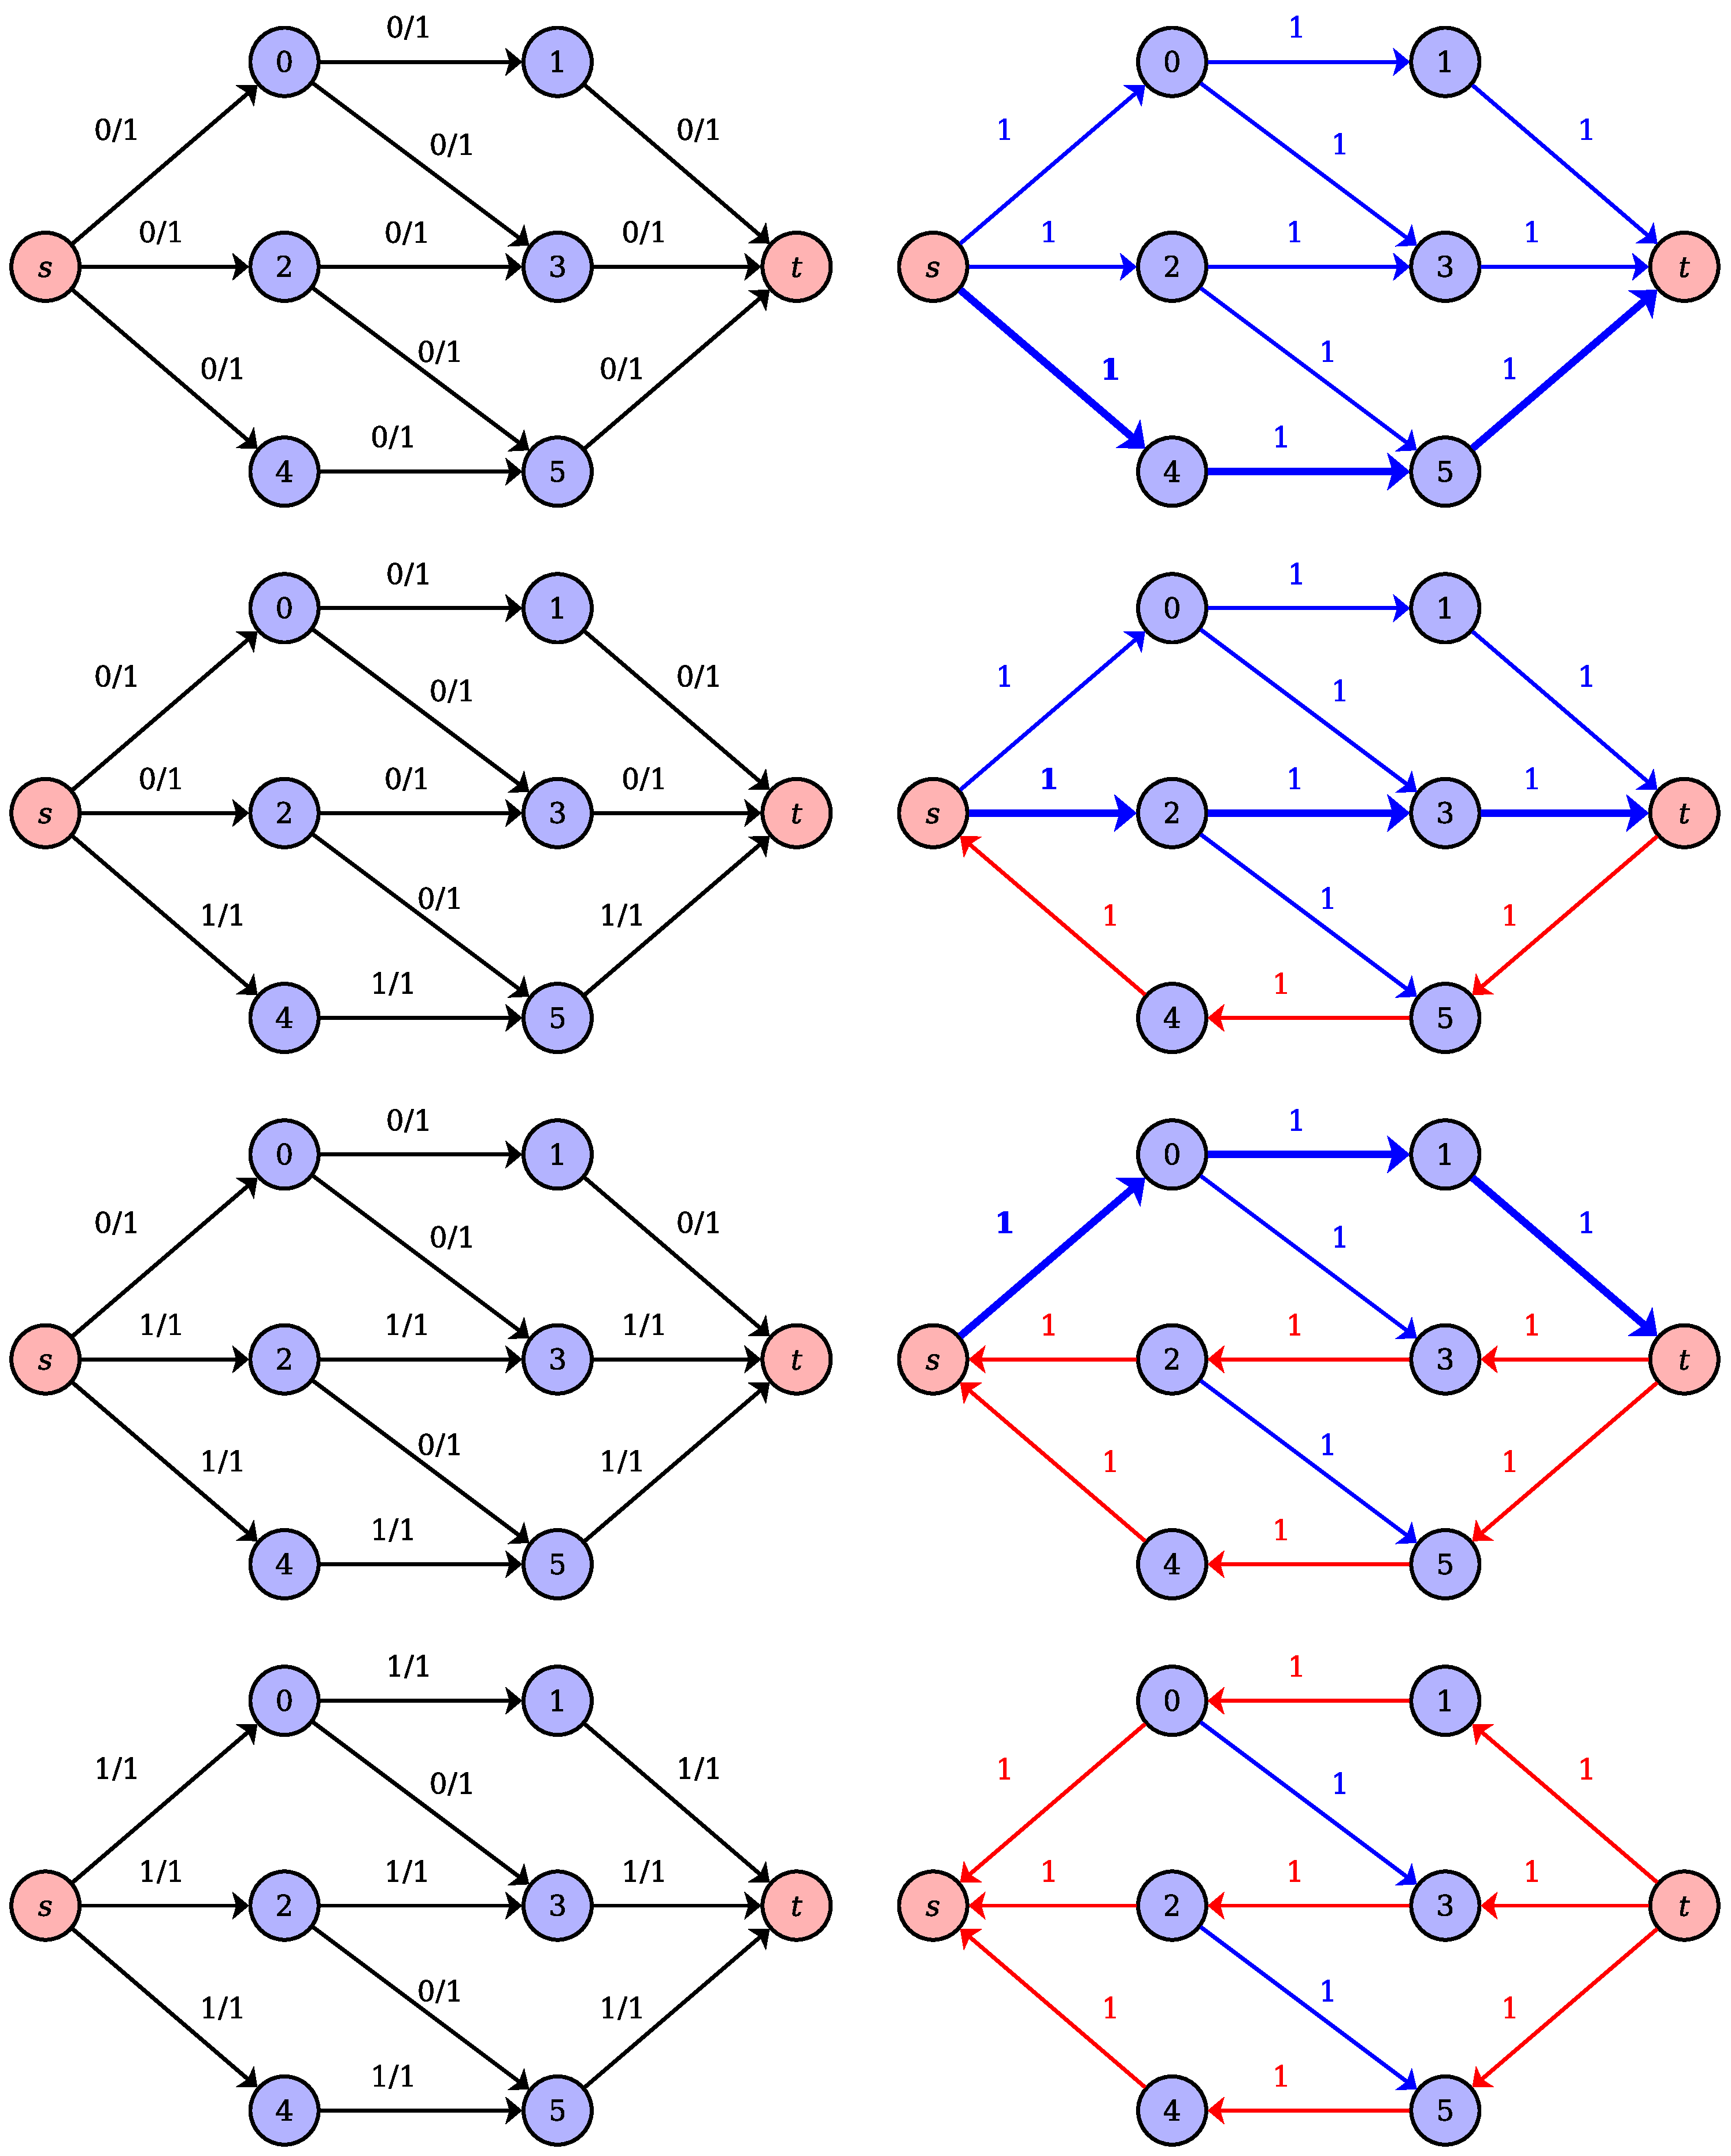
\includegraphics[width=0.75\linewidth]{Grafik/Diagramm2}
	\caption{Matching}
	\label{fig:Matching}
\end{figure}
In diesem Fall handelt es sich um ein Matching Problem. Wir haben die beiden Partitionen $A:=\{0,2,4\}~~B:=\{1,3,5\}$. Die lässt sich durch folgende Feststellungen belegen:
\begin{itemize}
	\item Es gibt nur Pfade von $A$ nach $B$
	\item Es gibt keine Pfade innerhalb von $A$ oder $B$
	\item $s$ ist mit allen Knoten aus $A$ verbunden und zu $t$ führen nur Kanten aus $B$
\end{itemize}
Entfernt man die Knoten $s$ und $t$, sowie alle mit diesen verbunden Kanten, erhält man einen bipartiten Graphen. Entfernt man nun noch alle Kanten mit einem Durchfluss von $0$ und macht aus den gerichteten Kanten ungerichtete, hat man ein maximales Matching.
\subsection*{Zusatzaufgabe: ResidualGraph.java}
\lstinputlisting[style=java,basicstyle=\scriptsize\ttfamily]{Code/ResidualGraph.java}
%\clearpage
%$ $
%\clearpage
\subsection*{Zusatzaufgabe: ResidualGraph.java}
\lstinputlisting[style=java,basicstyle=\ttfamily\scriptsize]{Code/ResidualGraph.java}
\end{document}